%        File: stochastic_methods.tex
%     Created: Mon Jun 08 03:00 PM 2009 C
% Last Change: Mon Jun 08 03:00 PM 2009 C
%



\documentclass[letterpaper,10pt]{article} 
\usepackage[pdftex]{color,graphicx} 
\usepackage{amsmath, amsfonts, amssymb, latexsym, inputenc, moreverb, wrapfig, subfigure, array, lscape, setspace, cite}
\usepackage[pdftex, colorlinks]{hyperref}
\newcommand{\ud}{\mathrm{d}} 
\newcommand{\degree}{$^{\circ}$}
\newcommand{\tb}[1]{\textcolor{blue}{#1}} 
\newcommand{\E}{\text{E}}

%\usepackage{fullpage} %% 1 inch margins by default
%\usepackage{pslatex}  %% use normal postscript fonts (like times new roman)

\title{Stochastic Methods for Ecology and Evolution}
\author{Carl Boettiger}
\begin{document}
\maketitle

% It begins.  Here I am at IIASA, beginning of the second week, but almost the first chance I have to settle down and do some real work -- 8 June, 2009.  This is meant to be a collection of methods to calculate certain quantities from stochastic processes, the applications of which form the bulk of the problem I will address this summer.  

% The organization of these ideas has yet to be developed -- whether by model, mathematical method, or biological problem.  

\section{Extinction Probabilities}

Gardiner (1985).  

We consider single-step birth death models for the majority of this work.  Though they will become multidimensional in later parts of the work, as we deal with multiple species or explicit environmental changes, for the time being we will focus on the one-dimensional bith-death process.  The Markov process is defined over positive integers, $n \in \mathbb{Z}^+$, and will sometimes be assumed to be bounded above by some integer $N$.  The process is determined by two state-dependent rates, $b(n)$ and $d(n)$, as depicted in Figure~\ref{fig:markov}.  

\begin{figure}[h]
\begin{center}
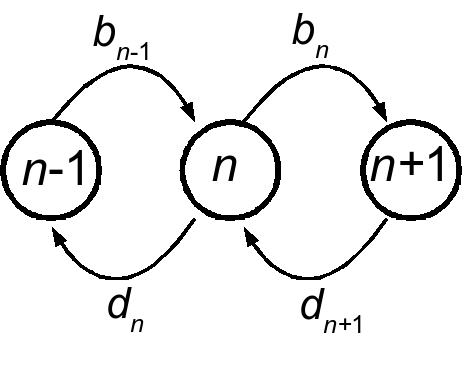
\includegraphics[width=.4\textwidth]{images/markov}
\end{center}
\caption{The birth-death Markov process}
\label{fig:markov}
\end{figure}

The process is specified by the Master equation:

\begin{equation}
\frac{\partial P(n,t)}{\partial t} = b(n-1)P(n-1,t)+d(n+1)P(n+1) - \left( b(n) + d(n)  \right) P(n)
\label{mastereq}
\end{equation}

and approximated by the method of Kurtz (1971) or van Kampen's linear nois expansion as:

\begin{equation}
\frac{\partial P(\tilde n,t)}{\partial t} = - \underbrace{\frac{\partial \left( b(\tilde n)-d(\tilde n) \right)}{\partial \tilde n}}_{A(\tilde n) } \frac{\partial}{\partial \tilde n} \tilde n  P(\tilde n,t)+ \underbrace{\frac{b(\tilde n)+ d(\tilde n)}{2} }_{B(\tilde n)/2} \frac{\partial^2}{\partial \tilde n^2} P(\tilde n)
\label{forward}
\end{equation}

Note that $n\to \tilde n$ where $\tilde n \in \mathbb{R}$ has become a continuous value in the limit of large system size.  The coefficients $A(x)$ and $B(x)$ are the jump moments $\partial_x \alpha_{1,0}(x)$ and $\alpha_{2,0}(x)$ in the van Kampen expansion.  This expression is known as the forward Kolmogrov equation.  Its solution is a Guassian, with mean and variance given respectively by

\begin{align}
\frac{\ud x }{\ud t} &= b(x)-d(x) \nonumber \\
\frac{\ud \sigma^2}{\ud t} &= A(x) \sigma^2 + B(x)
\label{moments}
\end{align}



Related to~\eqref{forward} is the backward Kolmogrov equation which we use for first-passage time problems:

\begin{equation}
\frac{\partial P(\tilde n,t)}{\partial t} = A(\tilde n) \frac{\partial}{\partial \tilde n}  P(\tilde n,t)+ \tfrac{1}{2}  B(\tilde n)\frac{\partial^2}{\partial \tilde n^2} P(\tilde n)
\label{backward}
\end{equation}

From this we have the first passage time starting at $x$ across an absorbing boundary $a < b$ given $b$ is reflecting:

\begin{equation}
T(x) = 2 \int^x_a \frac{\ud y}{\psi(y)} \int_y^b \frac{\psi(z) }{B(z)} \ud z
\label{firstpassage}
\end{equation}
where we define the integrating factor 
\begin{equation}
\exp\left( \int_a^y \ud x \left[ \frac{2 A(x)}{B(x)} \right] \right)
\label{integrating factor}
\end{equation}

It is useful to work these results out for some familiar models.  
\subsubsection*{Levins Model}
We first consider the Levins model:
\begin{align}
b(n) &= c n \left( 1 - n/K \right) \nonumber \\
d(n) &= e n
\label{levins}
\end{align}

$K$ is the number of patches, and also the convenient measure of system size.  In the limit of large $K$, $\tilde n = \tfrac{n}{K}$ represents the fraction of occupied patches, and we have the coeffients:
\begin{align*}
& A(\tilde n) = c(1-2 \tilde n)-e \\
& B(\tilde n) = c \tilde n (1 - \tilde n) + e \tilde n
\end{align*}

By way of~\eqref{moments} we have the equilibrium mean and variance:
\begin{align*}
& \langle \tilde n \rangle = 1-\frac{e}{c} \\
& \langle (\tilde n - \langle \tilde n \rangle )^2 \rangle = \frac{e}{c}
\end{align*}

\subsubsection*{Logistic Model}
A closely related model is the logistic with the following interpretation:
\begin{align*}
& b(n) = r n \\
& d(n) = \frac{r n^2}{K}
\end{align*}
Which has mean and variance both equal to $K$, and coefficents:
\begin{align*}
& A(x) = r  - \frac{2 r x}{K} \\
& B(x) = rx + \frac{rx^2}{K}
\end{align*}


\end{document}


